%Layout
	\documentclass[a4paper, twocolumn, twoside, 11pt]{article}
	\setlength{\columnsep}{1cm}
	\setlength{\parskip}{6pt}
	%\usepackage{geometry}
	\usepackage[margin=1.5cm]{geometry}
	\usepackage{float}
	%\usepackage{multicol}
	\usepackage{tocloft}
	\renewcommand\cftsecafterpnum{\vskip-5pt}
	%\usepackage{hyperref}
	\usepackage{enumitem}
	\usepackage[toc,page]{appendix}

%fonts
	\usepackage[T1]{fontenc}
	\usepackage[sfdefault]{roboto}
	\usepackage[T1]{fontenc}
	\usepackage[usenames, dvipsnames]{color}
	
%URLs
	\usepackage[colorlinks=true,
				linkcolor=black,
				urlcolor=WildStrawberry]{hyperref}

%Code listings
	
	\usepackage{listings}
	\definecolor{code}{rgb}{0.95,0.95,0.95}
	\definecolor{codeframe}{rgb}{0.9,0.9,0.9}
	
	\lstset{
		frame=single,
		numbers=left,
		numbersep=10pt,
		tabsize=8,
		basicstyle=\footnotesize\ttfamily,
		rulecolor=\color{codeframe},
		backgroundcolor=\color{code}
		}

	%Python Specific
	\definecolor{pcomment}{RGB}{207,0,19}
	\definecolor{pkey}{RGB}{241,117,34 }
	\definecolor{pcode}{rgb}{0.95,0.95,1.0}
	\definecolor{pcodeframe}{rgb}{0.8,0.8,1.0}
	\definecolor{codenumber}{rgb}{0.5,0.5,0.5}
	
	\lstdefinestyle{python}{
		language=Python,
		rulecolor=\color{pcodeframe},
		backgroundcolor=\color{pcode},
		keywordstyle=\color{pkey},
		commentstyle=\color{pcomment},
		numberstyle=\tiny\color{codenumber},
		emphstyle=\color{purple},
		showstringspaces=false,
		tabsize=4,
		breaklines=true
		}
%Asides
	\usepackage{mdframed}
	\newenvironment{aside}
		{
		\begin{mdframed}[
			style=0,%
			leftline=false,
			rightline=false,
			innerbottommargin=2pt,
			innerleftmargin=12pt,
			innerrightmargin=0pt,
			linewidth=0.75pt,
			skipabove=6pt,
			skipbelow=6pt
			]
				\small
				\color{JungleGreen}
				\setlength{\parskip}{2pt}
				\vspace{2pt} %correct for parskip
		}
		{
		\end{mdframed}
		}

%Everything else
	\usepackage[utf8]{inputenc}
	\usepackage{graphicx}
	
%	-	-	-	-	-	-	-	-	-	-	-	-	-	-	-	-	-	-	-	-

\begin{document}

	\author{Manchester Raspberry Jam}
	\title{Workshop 11: GPIO \& Motors}
	\date{}

	\maketitle
	
	\setcounter{tocdepth}{1}
	\tableofcontents
	
	%	-	PART 0
	\setcounter{section}{-1}
	\section{Introduction}
	
		The workshop shows how to control a motor with the Raspberry Pi, using a breadboard circuit and a standard motor controller chip. The motor is then programmed with the Python GPIO library.

		This is and introductory workshop and is suitable for anybody to attempt.
		
		These booklets were created using {\fontfamily{rfdefault}\selectfont \LaTeX}, an advanced typesetting system used for several sorts of books, academic reports and letters. The schematic diagrams were created using \textit{Fritzing}, a free hardware prototyping and PCB design software.
		
		To allow modification and redistribution of these booklets, they are distributed under the CC BY-SA 4.0 License.
	
		\subsection*{What you'll need}
			
			The hardware requirements for this workshop are listed below. %Illustrations are provided on page \textbf{REF} below.
	
			\begin{itemize}[noitemsep]		
				\item A solderless breadboard, preferably one with seperate bus strips. (those labelled + \& -)
				\item Male-to-female \& male-to-male jumper cables.
				\item A 6V DC motor.
				\item A L293D or L293DNE motor controller.
				\item (Optional) a 4$\times$AA Battery Pack				
			\end{itemize}
			
			\newpage
			
			For the LED exercise in \autoref{sec:LED}, you will also require:
			
			\begin{itemize}[noitemsep]	
				\item An LED
				\item A $\sim 330 \Omega$ Resistor
			\end{itemize}
				
			You can download both the template and completed python scripts for this workshop at \url{bit.ly/mcrraspjam}, along with a PDF copy of these notes.
			
			All required APIs are pre-installed with Raspbian.
			
	
		\subsection*{Code listings \& asides}
	
			When you need to make changes to your code, they'll be presented in boxes like the following:

			\lstinputlisting[style=Python]{code/helloworld.py}
	
			You might not need to copy everything, so check the line numbers to make sure you're not copying something twice.
			
			Terminal commands are listed as such, copy everything \textit{after} the dollar sign. Lines without dollar signs are example outputs, and do not need to be copied.
			
			\begin{lstlisting}
$ cd code
$ python3 helloworld.py 
Hello, World!
Hello, World!
..
			\end{lstlisting}
		
		\subsection*{Questions?}
		
			Send any corrections, suggestions or questions to:
			\url{jam@jackjkelly.com}\label{email}
	
	
	%Main Sections	
 	\newpage
	\section{A Simple LED Circuit}
\label{sec:LED}

	\subsection{Setting up the circuit}
	
		Let's start off with a simple circuit. Firstly, we'll always shut down and \textbf{unplug} our Pi before we begin connecting to the GPIO.
		
		We will build our circuit using a breadboard. Breadboards have conductive wire underneath their circuits, which form `lanes'. You can see these wires in figure \ref{fig:pinout_breadboard}.
	
		\begin{figure}[h]
			\centering
			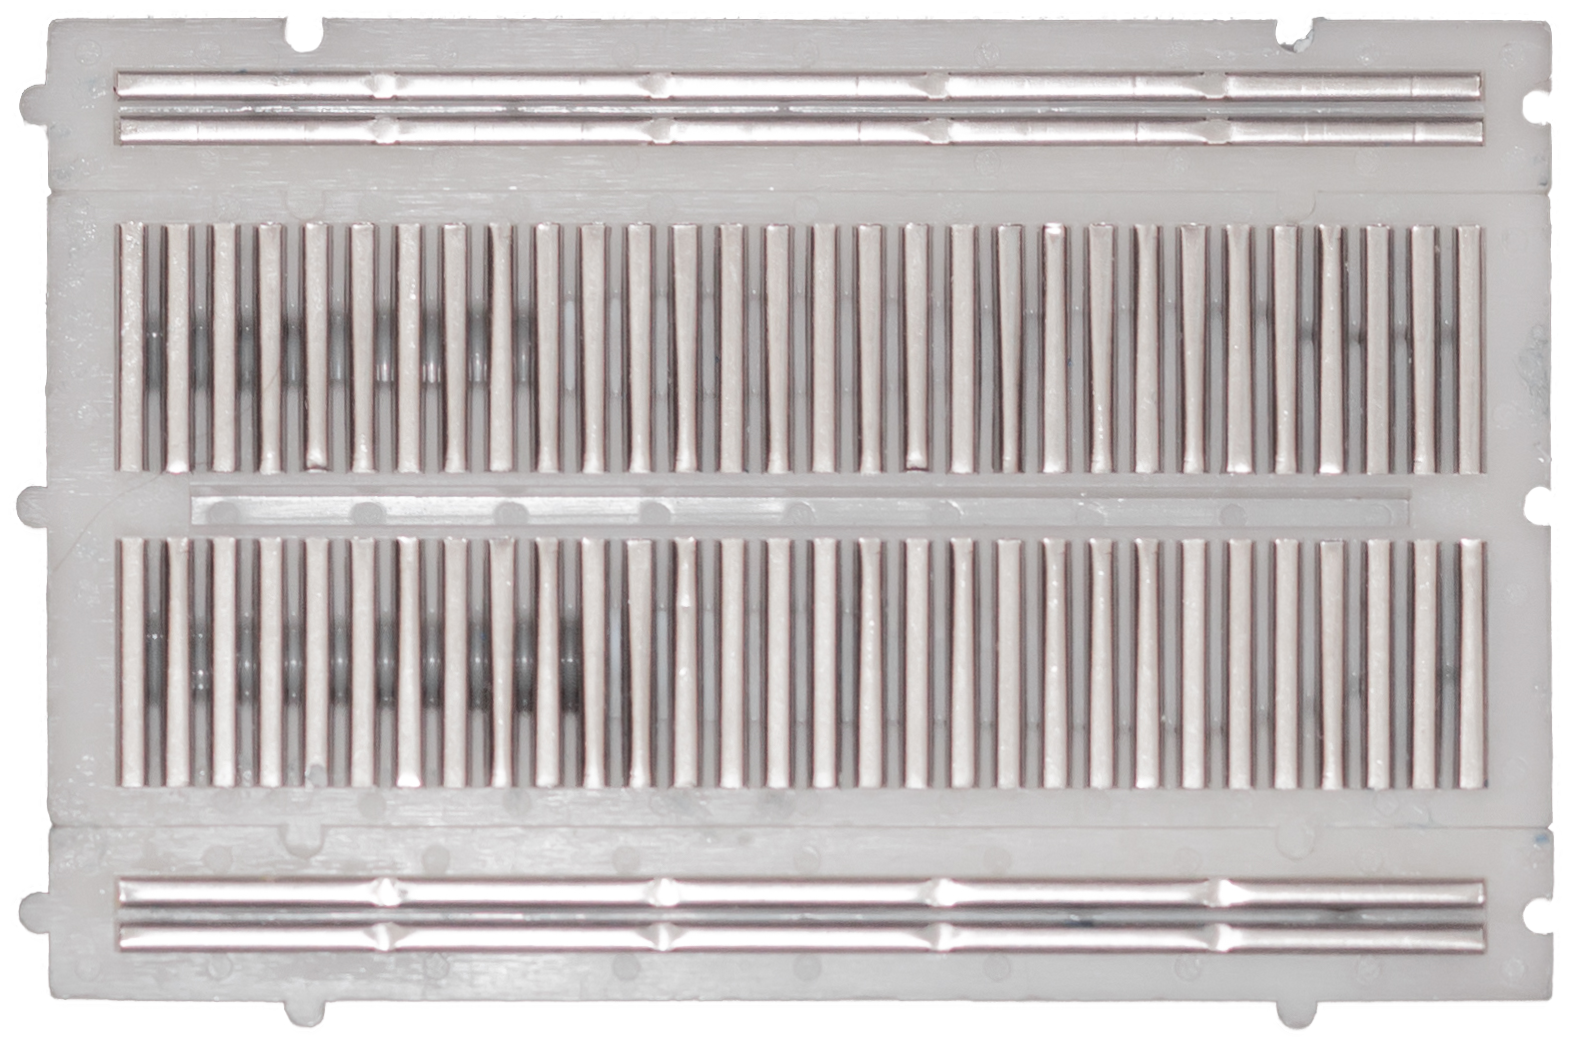
\includegraphics[width=0.75\linewidth]{img/breadboard_underside}
			\caption{The underside of a breadboard, showing the direction of electrical connections.}
			\label{fig:pinout_breadboard}
		\end{figure}
	
		We will use the positive and negative bus `lanes' like the ends of a battery in a simple electronic circuit, current starts at the positive end, and travels through components to the negative end.
		
		To make a complete circuit, we will connect these lanes to the Pi's GPIO.
		
		\begin{enumerate}[noitemsep]
			\item \textbf{Connect} the positive bus to the 3V3 pin on the Raspberry Pi with a jumper cable.
			\item \textbf{Connect} the negative bus to one of the GND pins with another jumper cable.
		\end{enumerate}
	
		By convention, you should use a red cable for the positive terminal and black for the negative terminal.
		
		\begin{enumerate}[noitemsep]
			\setcounter{enumi}{2}
			\item \textbf{Place} the LED across the gap in the centre of the breadboard, a pin on each side.
			\item Use a Jumper cable to \textbf{connect} the positive bus to the positive leg of the LED.
			\small
			\begin{itemize}[noitemsep]
				\item The LED is a Diode, so only lets current through one way.
				\item the positive leg (anode) of the LED is the longer of the two legs.
			\end{itemize}
			\normalsize
		\end{enumerate}
		
		We will now need to complete the circuit by connecting the negative pin of the LED.
		
		However, the LED will try and take a lot of power. To prevent it from burning out the Raspberry Pi, we'll add a resistor to limit the current flowing through the LED.
		
		\begin{enumerate}[noitemsep]
			\setcounter{enumi}{4}
			\item \textbf{Insert} the resistor in the lane where the negative LED leg is placed, and bridge it to any other lane.
			\item \textbf{Connect} this lane back to the negative bus with a jumper cable.
		\end{enumerate}
		
		\begin{figure}[h]
			\centering
			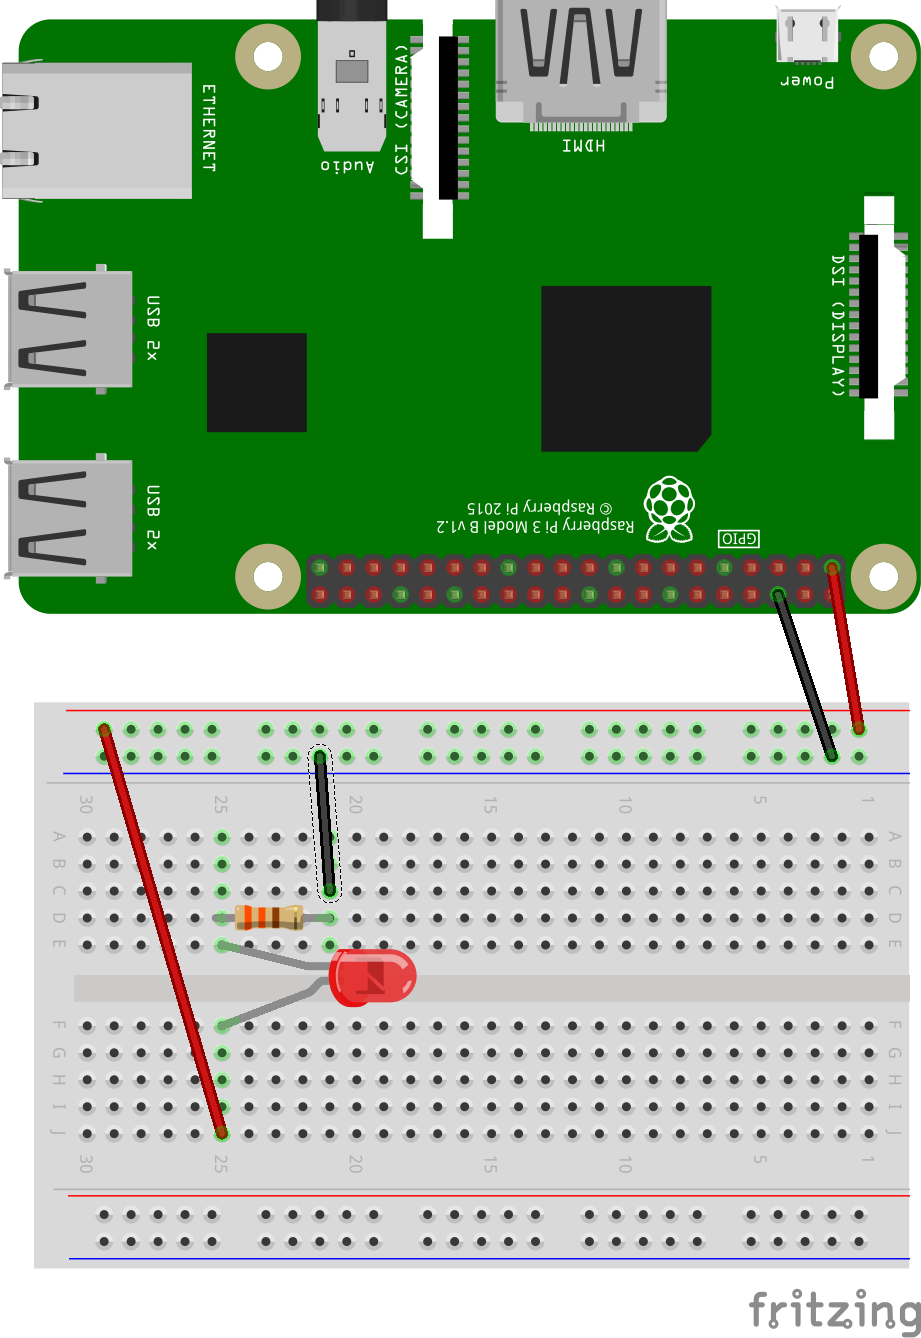
\includegraphics[width=0.5\linewidth]{img/schematic_LED_3}
			\caption{The complete LED circuit}
			\label{fig:schematic_LED_3}
		\end{figure}
		
		Once you're happy your circuit matches figure \ref{fig:schematic_LED_3}, you can try turning on your Raspberry Pi. If everything is correctly connected, your LED will light up!
		
	\subsection{Modify for GPIO}
	
			Our LED is currently connected to a constant 3.3 volt supply, so we are unable to turn the LED off without unplugging the whole Pi. To control the LED through code, we need to use a GPIO pin.
	
			\begin{enumerate}[nosep]
				\item Remember to shut down and \textbf{unplug} your Pi first.
				\item \textbf{Remove} the two red cables that were supplying the 3V3 voltage.
				\item Use a jumper cable to \textbf{connect} GPIO pin 23 to the positive pin of the LED.
			\end{enumerate}	
		
			\begin{figure}[h]
				\centering
				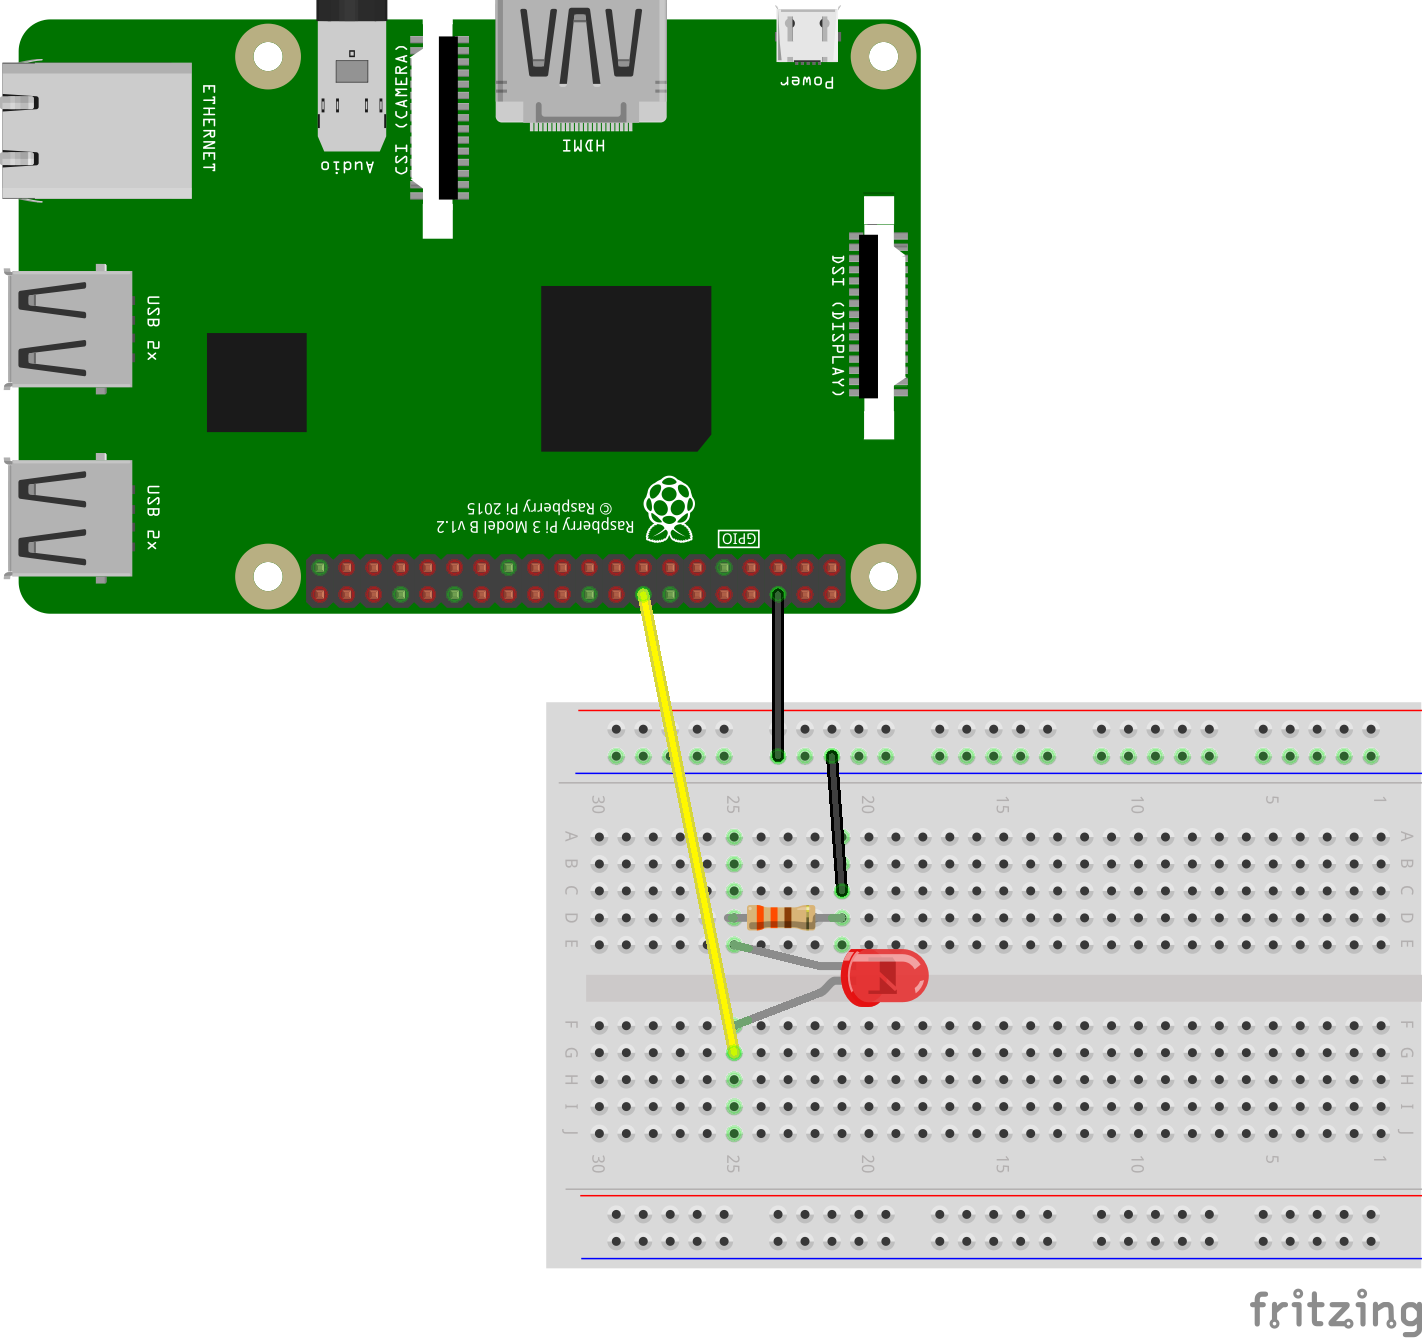
\includegraphics[width=0.6\linewidth]{img/schematic_LED_4}
				\caption{A GPIO controlled LED circuit}
				\label{fig:schematic_LED_4}
			\end{figure}
		
	\subsection{Programming the LED}
		
			Once you're happy again with the circuit, you can start you Pi up again.
			The LED will be off to begin with, so we will write a simple Python program to turn the LED on.
			
			Once your Pi is started up, start \textit{IDLE 3} and open the template python file for this workshop.
		
			\newpage
			\lstinputlisting[style=Python, lastline=6]{code/0_LED.py}
			
			Add the following lines into this file:
			
			\lstinputlisting[style=Python, firstline=7, firstnumber=7, lastline = 10]{code/0_LED.py}
			
			Before we control something through GPIO, we need to setup the pin. We just stated that pin 16 (labelled `LED') is an output device, i.e. we are outputting a signal to the light, we aren't reading a sensor input.
			
			Note the pin number is 16, not 23. We plugged into GPIO pin 23, but some pins on this block have other functionalities, but are still numbered. (See Appendix \ref{sec:pinout} for full pinout)
			
			Now it is set up, we can control the GPIO pin:
			
			\lstinputlisting[style=Python, firstline=11, firstnumber=11, lastline = 13]{code/0_LED.py}
			
			Once again, we are sending a command for pin number 16 (`LED'), this time telling it to output a `high' signal. This will turn on our LED.
			
			Let's have our LED on for a few seconds, then turn it off before the program ends. The function sleep() will cause the program to wait, then we will repeat the GPIO.output() function, this time using GPIO.LOW to turn off the LED.
			
			\lstinputlisting[style=Python, firstline=14, firstnumber=14, lastline = 20]{code/0_LED.py}
			
			We place GPIO.cleanup() at the end of our program, to reset the pin setup for the next program.
			
			You can now try running your program.
		

	\section{The Motor Circuit}
	
	\subsection{Motor Controller Chips}
		
		\textit{<Written explanation to be added after the workshop>}
		
		The pinout for the L293D/L239DNE is as follows:
		
		\begin{figure}[h]
			\centering
			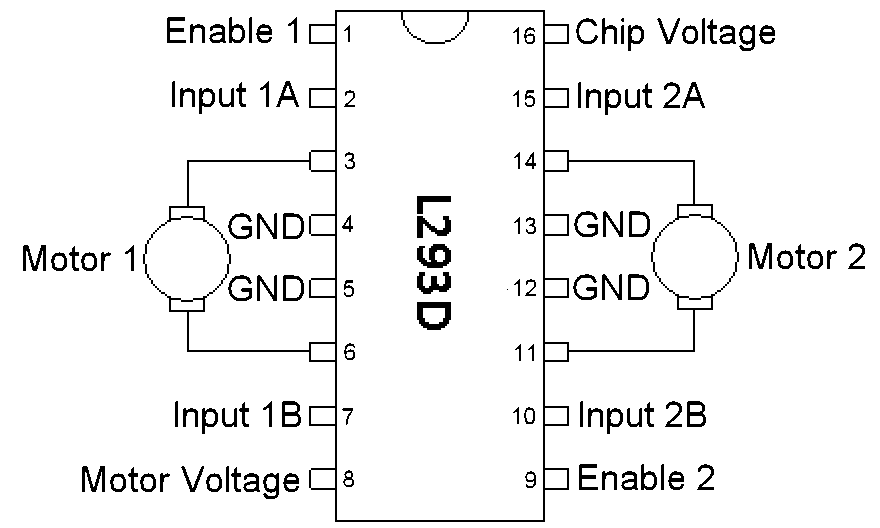
\includegraphics[width=0.7\linewidth]{img/pinout_L293DNE}
			\scriptsize
			\\ Source: \url{https://www.rs-online.com/designspark/raspberry-pi-controlling-a-motor-via-gpio}
			\normalsize
			\label{fig:pinout_L293DNE}
		\end{figure}

			
	\subsection{Setting up a Motor Circuit}
		
		Firstly, we'll ensure we have the motors and chip powered.
		
		\begin{enumerate}[noitemsep]
			\item Remember to shut down and \textbf{unplug} your Pi first.
			\item \textbf{Place} the L293DNE chip across the central gap, noting the orientation. In the illustration, the semicircle cutout is facing to the right.
			\item \textbf{Connect} both positive buses with a jumper cable to a 5V pin. 
			\item \textbf{Connect} the Motor voltage and Chip voltage pins with their closest positive bus.
			\item \textbf{Connect} at least two ground pins on the chip to the motor's negative bus.
			\item \textbf{Connect} at least two GND pins on the pi to the Motor negative bus.
		\end{enumerate}
		
		Your breadboard should now look like figure \ref{fig:schematic_3}. Now, we will add the GPIO inputs and motor.
		
		\begin{figure}[h]
			\centering
			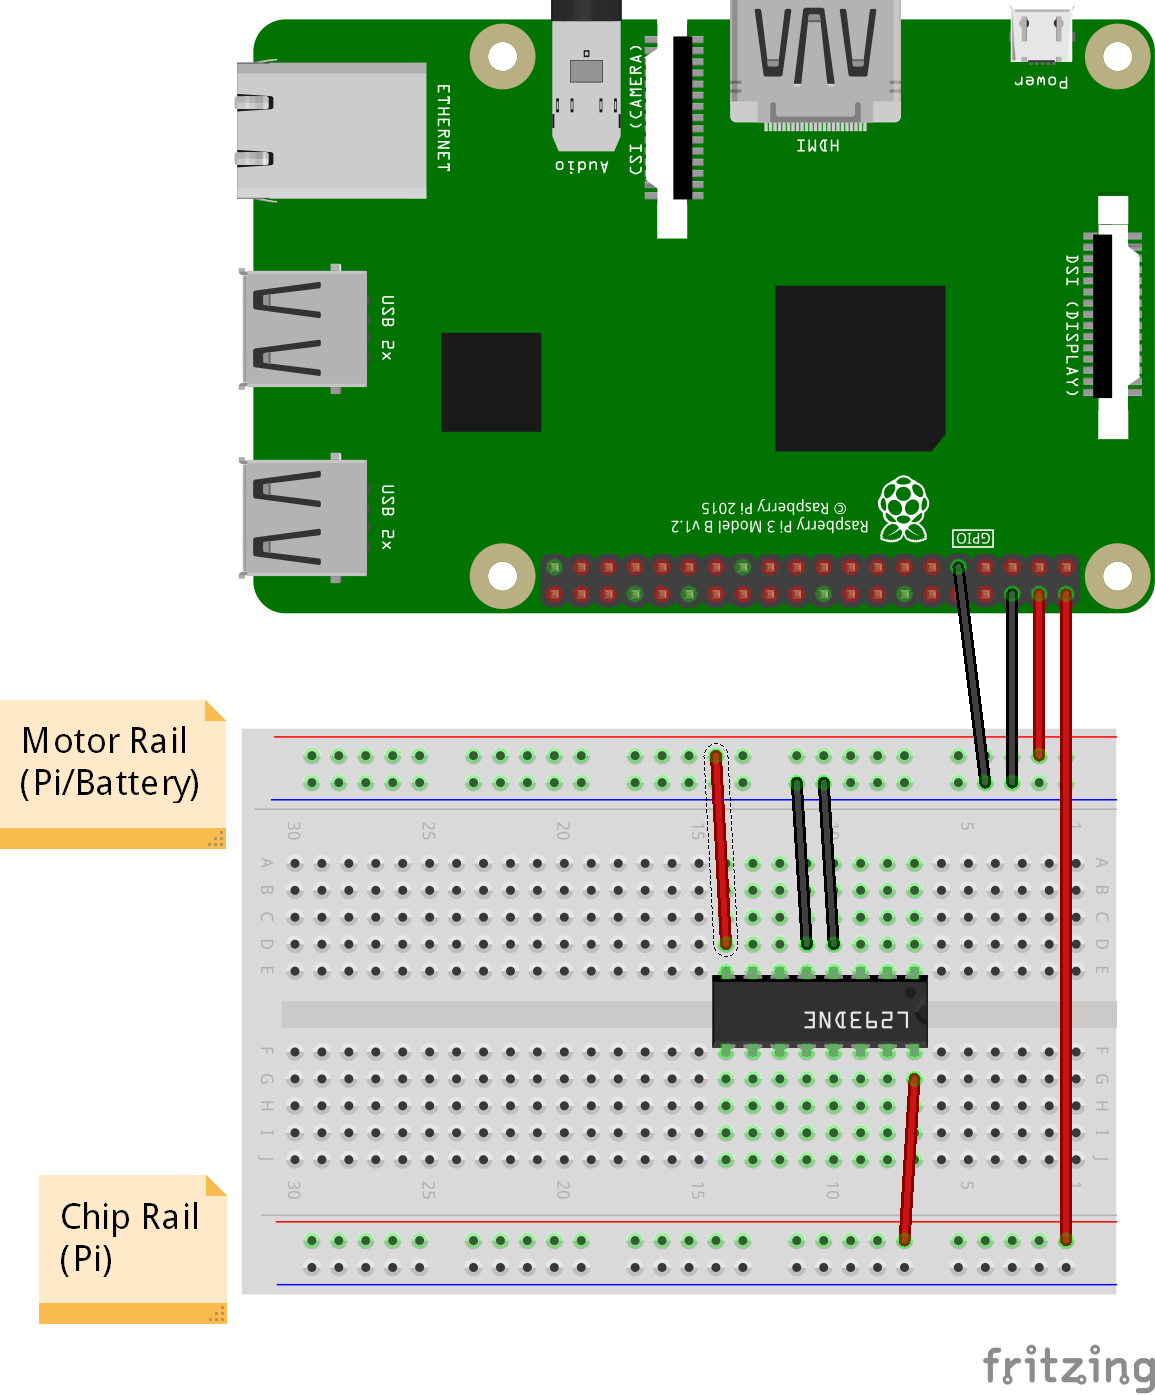
\includegraphics[width=0.6\linewidth]{img/schematic_3}
			\caption{Powering the L293DNE.}
			\label{fig:schematic_3}
		\end{figure}
		
		\begin{enumerate}[noitemsep]
			\setcounter{enumi}{6}
			\item \textbf{Connect} GPIO pin 23 to input 2A, and GPIO pin 24 to input 2B with a pair of jumper cables.
			\item \textbf{Connect} GPIO pin 25 to Enable 2 with another cable.
			\item \textbf{Connect} Connect the motor to the two motor pins (on the motor 2 side). \scriptsize \textit{If you don't have crocodile clips, try bending the pins of two jumper cables to keep them in place.} \normalsize
			\item \textbf{Connect} at least two GND pins on the pi to the Motor negative bus.
		\end{enumerate}
		
		If you're happy that your circuit is equivalent to the one shown in figure \ref{fig:schematic_5}, you can try turning on your Pi. If it makes it to the desktop, you probably haven't done anything too disastrous!
		
		\begin{figure}[h]
			\centering
			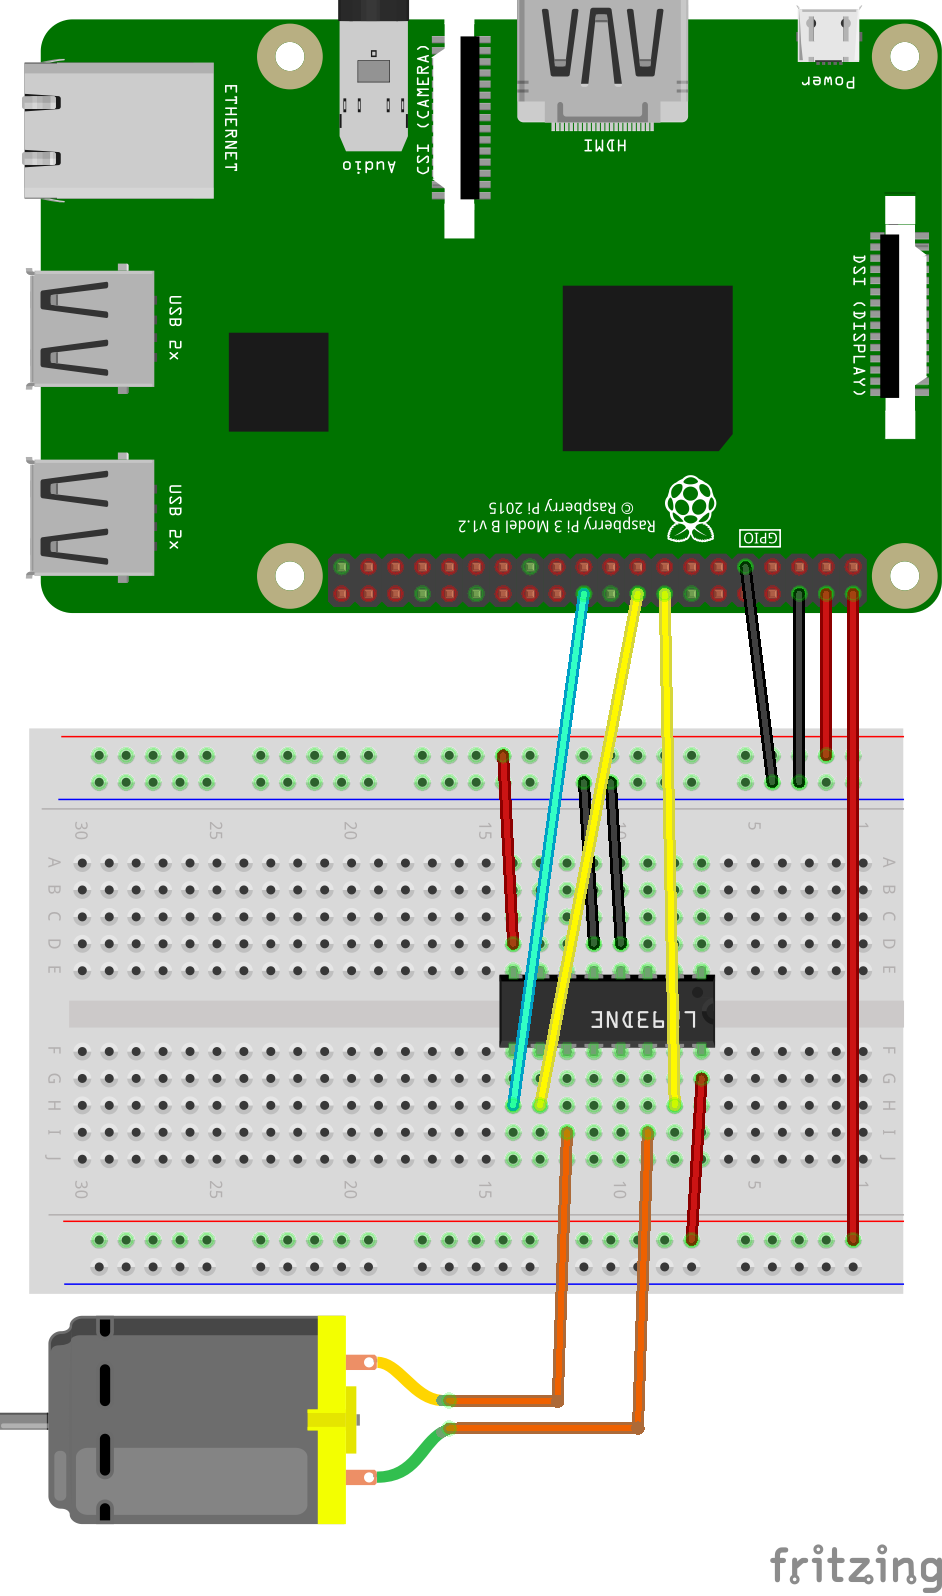
\includegraphics[width=0.6\linewidth]{img/schematic_5}
			\caption{The complete motor circuit.}
			\label{fig:schematic_5}
		\end{figure}
		
	\subsection{Programming the Motor}
	
		Start with a copy of the template program from before:
		
		\newpage		
		\lstinputlisting[style=Python, lastline=6]{code/1_Motor.py}
		
		This time, we will set up all three of the GPIO pins that we connected:
	
		\lstinputlisting[style=Python, firstline=7, firstnumber=7, lastline=15]{code/1_Motor.py}
		
		Remember that to turn on a motor, we need to set two opposing signals for A and B, then set enable to high. Therefore, to turn the motor on:
		
		\lstinputlisting[style=Python, firstline=16, firstnumber=16, lastline=20]{code/1_Motor.py}
		
		As with our LED, we will leave the motor running for a few seconds before turning it off. We do not need to change the A or B input, we can just change `Enable' to turn off the motor:
		
		\lstinputlisting[style=Python, firstline=21, firstnumber=21, lastline=26]{code/1_Motor.py}
		
		After adding the GPIO.cleanup() function, you can now try running your program.
		
		Make sure your motor is connected, and hold onto the body of the motor whilst running the program, as the motor likes to wiggle free of it's wires.
		
		\subsubsection*{Reverse Gear}
		
			One final thing to check. Our motor controller should allow us to run the motor in reverse. 
			
			Make the following changes to your program, and have a go at filling in the missing parameters for the GPIO.output function calls:
				
			\newpage
			\lstinputlisting[style=Python, firstline=21, firstnumber=21, lastline=38]{code/2_Motor.py}
			
			It will be difficult to tell which way the motor is spinning with nothing attached, but it tends to make a slightly different noise when running in the other direction.
			
			To double check, you can try placing some Blu Tack on the motor shaft and shaping it to make the spin more obvious.
			
			Congratulations on getting your motor working!
			
	%\newpage
	
	\begin{appendices}
		
	%Don't list each appendix in Table of Contents
	\addtocontents{toc}{\setcounter{tocdepth}{-1}}	
		
	\section{Completed Code Listings}
	
		\subsection*{0\_LED.py}
			\lstinputlisting[style=Python]{code/0_LED.py}
		\newpage
		\subsection*{1\_Motor.py}
			\lstinputlisting[style=Python]{code/2_Motor.py}	
			
	\section{GPIO Pinout (GPIO.BOARD)}
	
	\begin{figure}[h]
		\label{sec:pinout}
		\centering
		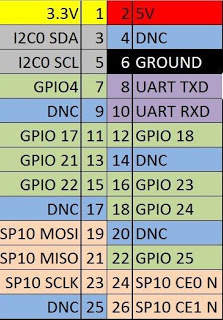
\includegraphics[width=0.5\linewidth]{img/pinout_pi}
		\scriptsize
		\\Source: \url{hobbytronics.co.uk/raspberry-pi-gpio-pinout}
		\normalsize
		\label{fig:pinout}
	\end{figure}
	\end{appendices}

\end{document}